\section{Overlap Analysis}
In order to calibrate the PCAL unit of the CLAS12 detector, one can think of dividing each PCAL module based on the 
overlapping shapes. One can either consider on the pixel level, where the pixel is a shape formed when all 
all the views are superimposed together or the calibration can be done by considering the strips of one 
view binned in the number of strips in the view which is to be calibrated. Although in general a three layer 
correlated pixel can be odd shaped, a two layer correlation can be straight forward. This section deals with the 
latter case. The general idea is to get the ADC readout pertaining to that overlap shape which is at a certain 
distance from the PMT corresponding to the strip for that particular view. These signals are fit to extract the 
centroids which are further fit as an exponential function of distance to get the calibration coefficients 
or the attenuation coefficients. 

\FloatBarrier
\subsection{Overlap Distance Measurement}
An important parameter in the calibration process is the measurement of distances of the overlap shapes. 
As previously mentioned, the distances are measured from the PMTs. Therefore from the known width of each 
scintillator strip and the number of strips in between an overlap shape and the readout end, it is 
straightforward to calculate the distances for each overlap shape by simple trigonometry. This idea, 
however, assumes that all the strips are of equal width and neglects any physical gap (if any) between strips.

The two layer correlation creates trapezoidal bins formed by the overlap of two different 
strip orientations\footnote{All of the studies in this section were primarily focused on the U-strip 
attenuations, rather than the V or W strips.}. An example of one of these trapezoids outlined in black can be 
seen in figure \ref{fig:trapezoidUWintersection}. Each one of these trapezoids should have a ADC readout value. The width 
of this physical bin can be found by
\begin{eqnarray}
 s = \frac{w}{\sin{\alpha}}    \nonumber\\
\Rightarrow s = \frac{w}{\cos{\beta}},
\end{eqnarray}
where $w$ is a single scintillator strip width ($\approx 4.5$cm) and $\alpha = 62.88904^0$. Statistically one might expect some 
sort of peak describing the distribution of values. The centroid of this distribution is used as a data point 
at that center of that physical bin.
\begin{figure}[t]
\centering
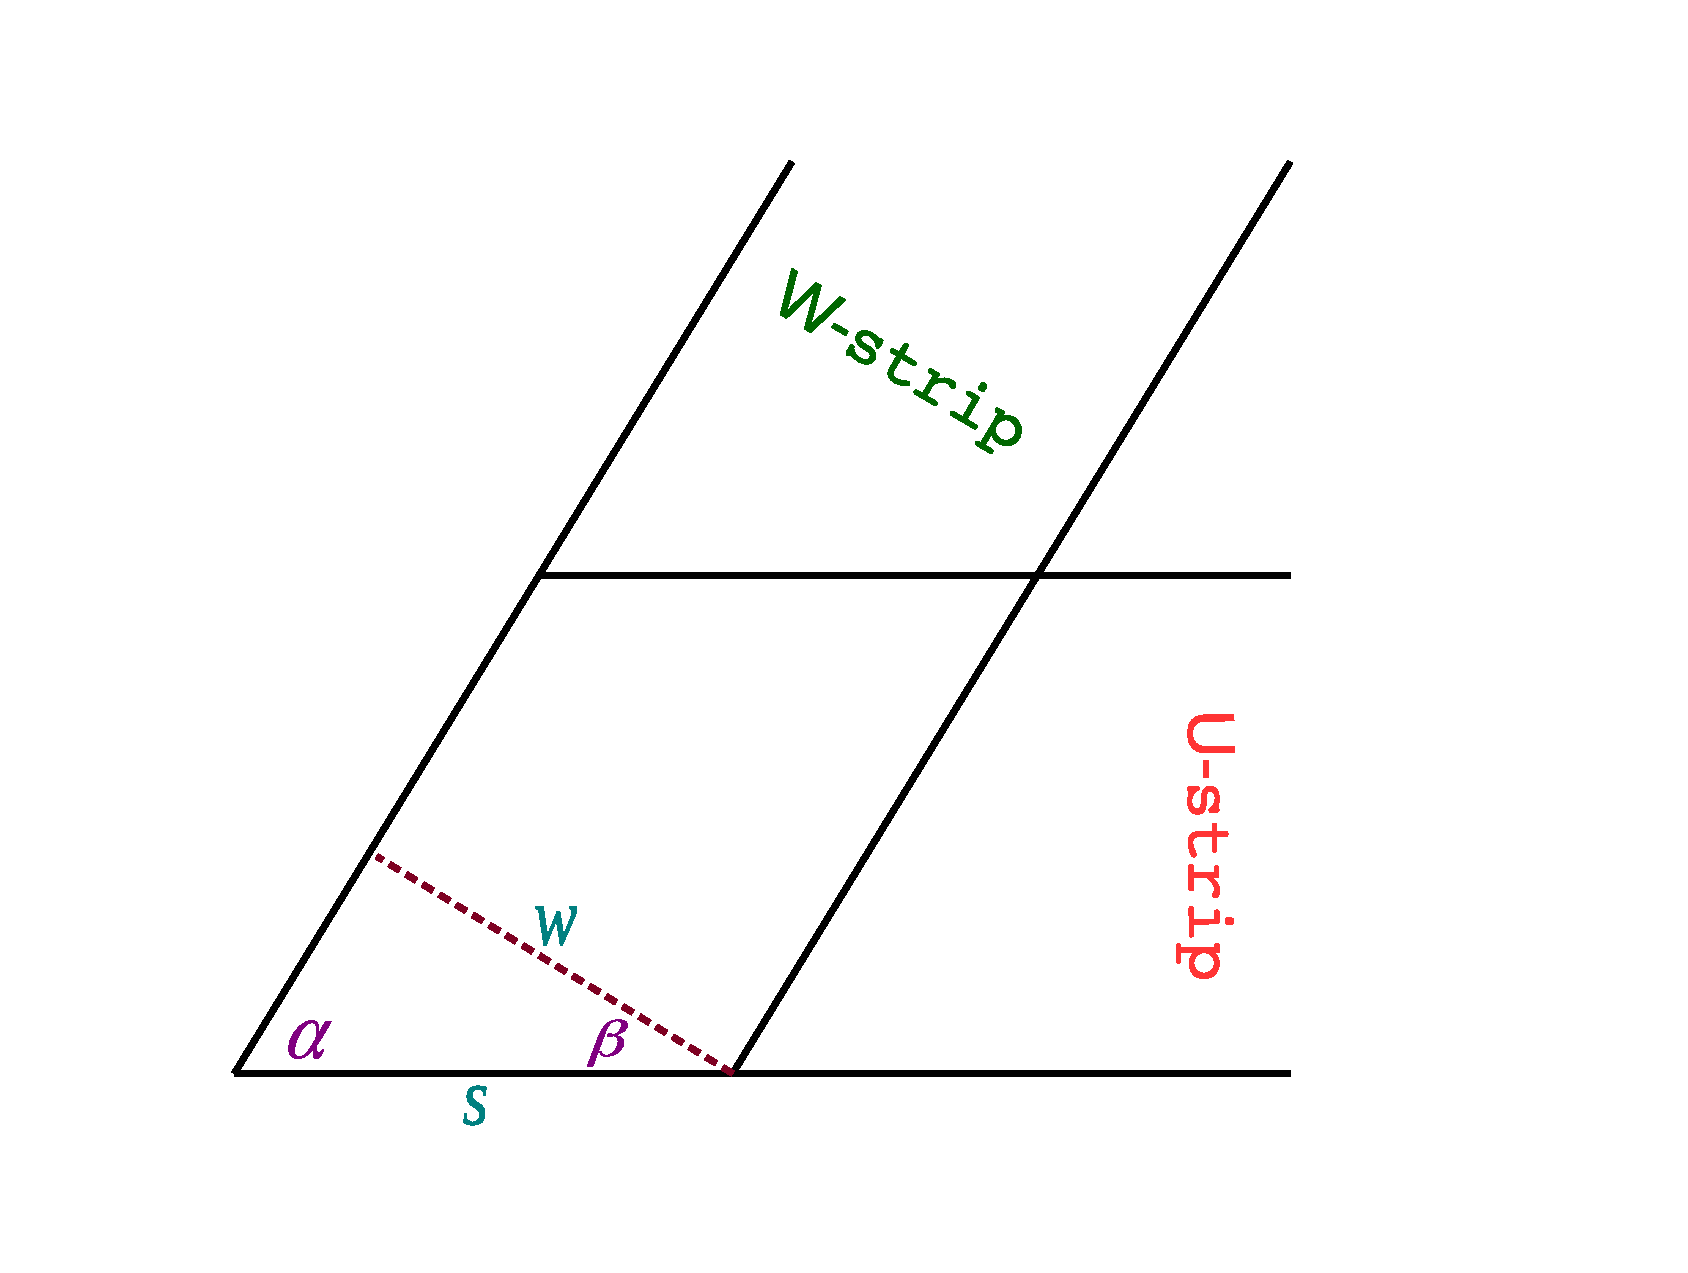
\includegraphics[width= 4in, keepaspectratio = true]{trapezoidUWintersection}
\caption{Shown is an outline of a generic intersection of a U and W strip. The distance between the trapezoidal area and the 
PCAL edge can be represented by a linear function of $s$.}
\label{fig:trapezoidUWintersection}
\end{figure}
\FloatBarrier

\clearpage
